\documentclass[12pt]{article}
\usepackage[margin=2.5cm]{geometry}
\usepackage{enumerate}
\usepackage{amsfonts}
\usepackage{amsmath}
\usepackage{fancyhdr}
\usepackage{amsmath}
\usepackage{amssymb}
\usepackage{amsthm}
\usepackage{mdframed}
\usepackage{graphicx}
\usepackage{subcaption}
\usepackage{adjustbox}
\usepackage{listings}
\usepackage{xcolor}
\usepackage{booktabs}
\usepackage[utf]{kotex}
\usepackage{hyperref}

\definecolor{codegreen}{rgb}{0,0.6,0}
\definecolor{codegray}{rgb}{0.5,0.5,0.5}
\definecolor{codepurple}{rgb}{0.58,0,0.82}
\definecolor{backcolour}{rgb}{0.95,0.95,0.92}

\lstdefinestyle{mystyle}{
    backgroundcolor=\color{backcolour},
    commentstyle=\color{codegreen},
    keywordstyle=\color{magenta},
    numberstyle=\tiny\color{codegray},
    stringstyle=\color{codepurple},
    basicstyle=\ttfamily\footnotesize,
    breakatwhitespace=false,
    breaklines=true,
    captionpos=b,
    keepspaces=true,
    numbers=left,
    numbersep=5pt,
    showspaces=false,
    showstringspaces=false,
    showtabs=false,
    tabsize=1
}

\lstset{style=mystyle}

\pagestyle{fancy}
\renewcommand{\headrulewidth}{0.4pt}
\lhead{CSC 343}
\rhead{Worksheet Solution}

\begin{document}
\title{CSC343 Worksheet Solution}
\maketitle

\bigskip


\begin{enumerate}[1.]
    \item \textbf{Exercise 2.2.1:} In fig 2.6 are instances of two relations that might
    constitute part of a banking exercise. Indicate the following

    \begin{center}
    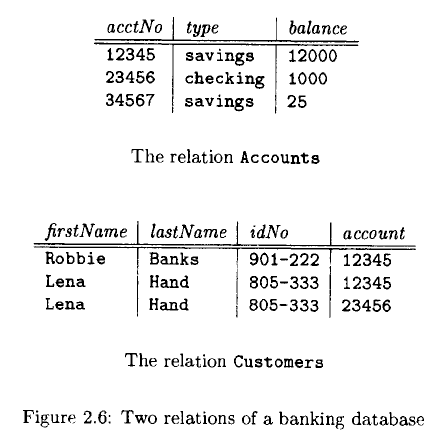
\includegraphics[width=0.6\linewidth]{images/worksheet_1_1.png}
    \end{center}

    \begin{enumerate}[a)]
        \item The attributes of each relation

        \begin{mdframed}
            \underline{\textbf{Answer:}}

            \bigskip

            \begin{itemize}
                \item Accounts: \textit{acctNo}, \textit{type}, \textit{balance}
                \item Customers: \textit{firstName}, \textit{lastName}, \textit{idNo}, \textit{account}
            \end{itemize}
        \end{mdframed}

        \bigskip

        \underline{\textbf{Notes:}}

        \bigskip

        \begin{itemize}
            \item \textbf{Attributes:} are the columns of a relation

            \begin{center}
            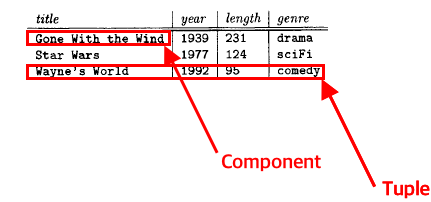
\includegraphics[width=0.8\linewidth]{images/worksheet_1_solution_1.png}
            \end{center}
        \end{itemize}

        \item The tuples of each relation

        \begin{mdframed}
            \underline{\textbf{Answer:}}

            \bigskip

            \begin{itemize}
                \item Accounts
                \begin{enumerate}[1.]
                    \item 12345, savings, 12000
                    \item 23456, checkings, 1000
                    \item 34567, savings, 25
                \end{enumerate}
                \item Customers
                \begin{enumerate}[1.]
                    \item Robbie, Banks, 901-222, 12345
                    \item Lena, Hand, 805-333, 12345
                    \item Lena, Hand, 805-333, 23456
                \end{enumerate}
            \end{itemize}
        \end{mdframed}

        \bigskip

        \underline{\textbf{Notes:}}

        \begin{itemize}
            \item \textbf{Tuple:} the rows of a relation, other than the header row
            containing the attribute names, are called tuples.
            \item A tuple has \underline{one \textbf{component}} for each attribute

            \begin{center}
            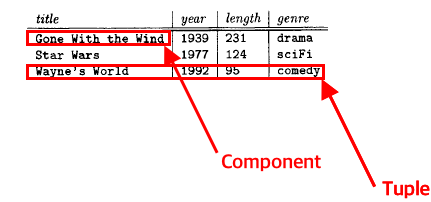
\includegraphics[width=0.8\linewidth]{images/worksheet_1_solution_2.png}
            \end{center}
        \end{itemize}

        \item The components of one tuple from each relation
        \begin{mdframed}
            \underline{\textbf{Answer:}}

            \begin{enumerate}[1.]
                \item Accounts
                \begin{itemize}
                    \item 12345
                \end{itemize}
                \item Customers
                \begin{itemize}
                    \item Robbie
                \end{itemize}
            \end{enumerate}

        \end{mdframed}
        \item The database schema

        \begin{mdframed}
            \underline{\textbf{Answer:}}

            \begin{enumerate}[1.]
                \item Accounts(acctNo, type, balance)
                \item Customers(firstName, lastName, idNo, account)
            \end{enumerate}
        \end{mdframed}

        \bigskip

        \underline{\textbf{Notes:}}

        \begin{itemize}
            \item \textbf{Schema:} Is the name of relation and the set of attributes
            for a relation

            \begin{itemize}
                \item e.g. Movies(title, year, length, genre)
            \end{itemize}
        \end{itemize}

        \item A suitable domain for each attribute

        \bigskip

        \begin{mdframed}
            \underline{\textbf{Answer:}}

            \begin{enumerate}[1.]
                \item Accounts (acctNo: integer, type: string, balance: integer)
                \item Customers (firstName: string, lastName: string, idNo: String, account: integer)
            \end{enumerate}
        \end{mdframed}

        \underline{\textbf{Notes:}}

        \begin{itemize}
            \item \textbf{Domain:} Is the elementary type of attributes in a
            relation Schema

            \begin{itemize}
                \item e.g. Movies(title: string, year: integer, length: integer, genre: string)
            \end{itemize}
        \end{itemize}
        \item Another equivalent way to present each relation

        \begin{mdframed}
            \underline{\textbf{Answer:}}

            \bigskip

            \begin{itemize}
                \item Account

                \begin{tabular}{|c|c|c|c|}
                    \hline
                    type & acctNo & balance\\
                    \hline
                    savings & 12345 & 12000\\
                    \hline
                    savings & 34567 & 25\\
                    \hline
                    checkings & 23456 & 1000\\
                    \hline
                \end{tabular}

                \item Customers

                \begin{tabular}{|c|c|c|c|}
                    \hline
                    account & idNo & lastName & firstName\\
                    \hline
                    12345 & 901-222 & Banks & Robbie\\
                    \hline
                    23456 & 805-333 & Hand & Lena\\
                    \hline
                    12345 & 805-333 & Hand & Lena\\
                    \hline
                \end{tabular}
            \end{itemize}
        \end{mdframed}

        \bigskip

        \underline{\textbf{Notes:}}

        \begin{itemize}
            \item Attributes along with its values in re-ordered form has the same relation as the original
            \item Tuples presented in different order has the same relation as the original

            \bigskip

            \begin{center}
            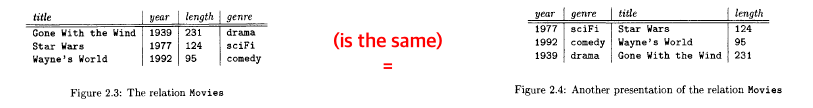
\includegraphics[width=\linewidth]{images/worksheet_1_solution_3.png}
            \end{center}
        \end{itemize}
    \end{enumerate}

    \item \textbf{Exercise 2.2.2:} In section 2.2.7 we suggested that there are many
    exmaples of attributes that are created for the purpose of serving as keys of
    relations. Give some additional examples.

    \bigskip

    \begin{mdframed}
        \underline{\textbf{Answer:}}

        \bigskip

        \begin{itemize}
            \item Account
            \begin{itemize}
                \item accoutNo
            \end{itemize}

            \item Customers
            \begin{itemize}
                \item firstName
                \item lastName
                \item idNo
                \item account
            \end{itemize}

        \end{itemize}
    \end{mdframed}


    \underline{\textbf{Notes:}}

    \begin{itemize}
        \item Attribute whose value is unique in each tuple or set of attributes
        whose combined values are unique

        \begin{center}
        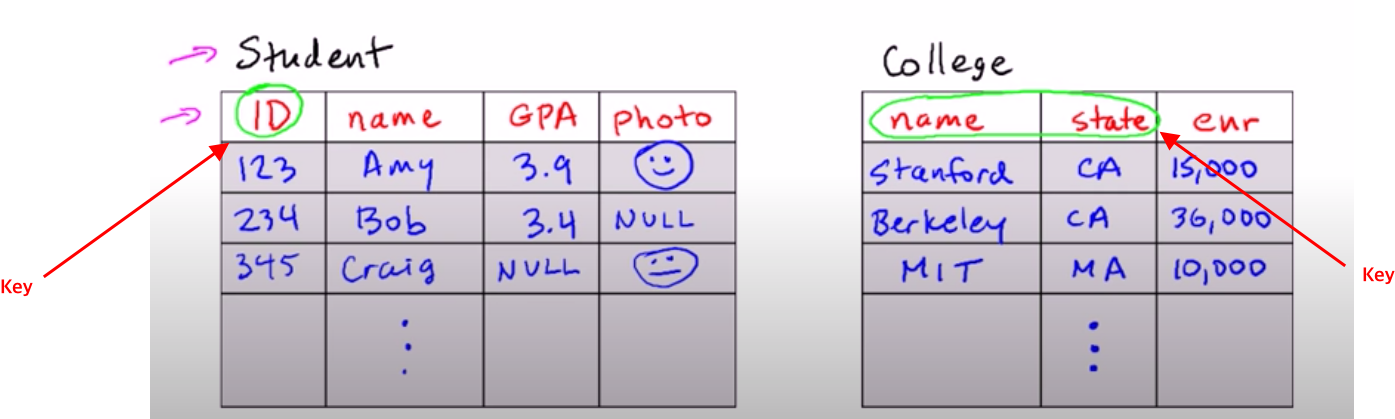
\includegraphics[width=\linewidth]{images/worksheet_1_solution_4.png}
        \end{center}
    \end{itemize}

    \item \textbf{Exericse 2.3.1} In this exercise we introduce one of our running
    examples of a relational database schema. The database schema consists of four relations,
    whose schemas are:

    \bigskip

    \begin{lstlisting}
    Product(maker, model, type)
    PC(model, speed, ram, hd, price)
    Laptop(model, speed, ram, hd, screen, price)
    Printer(model, color, type, price)
    \end{lstlisting}

    The \textbf{Product} relation gives the manufacturer, model number and type
    (PC, laptop, or printer) of various products. We assume for convenience that
    model numbers are unique over all manufactuers and product types; that assumption is
    not relaistic, and a real database would include a code for the manufacturer
    as part of the model number. The PC relation gives for each model number that
    is a PC the speed (of the processor, in gigahertz), the amount of RAM (in megabytes),
    the size of the hard disk (in gigabytes), and the price. The \textbf{Laptop}
    relation is similar, except that the screen size (in inches) is also included. The
    \textbf{Printer} relation records for each printer model wether the printer
    produces color output (true, if so), the process type (laser or ink-jet, typically),
    and the price.

    \bigskip

    Write the following declarations:

    \begin{enumerate}[a)]
        \item A suitable schema for relation \textbf{Product}

        \begin{mdframed}
            \underline{\textbf{Answer:}}

            \bigskip

    \begin{lstlisting}[language=SQL]
    CREATE TABLE Product (
        maker CHAR(100),
        model INT,
        type CHAR(7)
    );
    \end{lstlisting}

        \end{mdframed}


        \item A suitable schema for relation \textbf{Laptop}
        \item A suitable schema for relation \textbf{Printer}
        \item An alteration to your \textbf{Printer} schema from (d) to delete
        the attribute \textbf{color}
        \item An alternation to your \textbf{Laptop} schema from (c) to add the
        attribute \textbf{od} (optical-disk, e.g. cd or dvd). Let the default value
        for this attribute be `\textbf{none}' if the laptop does not have an optical
        disk.
    \end{enumerate}

    \item \textbf{Exericse 2.3.2} This exercise introduces another running example,
    concerning World War II capital ships. It involves the following relations:

    \bigskip

    \begin{lstlisting}
    Classes(class, type, country, numGuns, bore, displacement)
    Ships(name, class, launched)
    Battles(name, date)
    Outcomes(ship, battle, result)
    \end{lstlisting}

    \textbf{Ships} are bult in `classes' from the same design, and the class is
    usually named for the first ship of that class. The relation \textbf{Classes}
    records the name of the class, the type (`bb' for battleship or `bc' for battlecruiser),
    the country that built the ship, the number of main guns, the bore (diameter of
    the gun barrel, in inches) of the main guns, and the displacement (weight, in tones).
    Relation \textbf{Ships} records the name of the ship, the name of its class,
    and the year in which the ship was launched. Relation \textbf{Battles} gives
    the name and date battles involving these ships, and relation \textbf{Outcome}
    gives the result (sunk, damaged or ok) for each ship in each battle.

    \bigskip

    Write the following  declarations

    \bigskip

    \begin{enumerate}[a)]
        \item A suitable schema for relation \textbf{Classes}
        \item A suitable schema for relation \textbf{Ships}
        \item A suitable schema for relation \textbf{Battles}
        \item A suitable schema for relation \textbf{Outcomes}
        \item An alteration to your \textbf{Classes} relation from (a) to delete
        the attribute \textbf{bore}
        \item An alteration to your \textbf{Ships} relation from (b) to include
        attribute \textbf{yard} giving the shipard where the ship was built.
    \end{enumerate}
\end{enumerate}


\end{document}